\documentclass{article}

\usepackage[linesnumbered,boxed,ruled,commentsnumbered]{algorithm2e}
\usepackage{bm}
\usepackage{graphicx}
\usepackage{float}
\usepackage[bookmarks=true]{hyperref}
\usepackage{amsmath}
\begin{document}
\title{Deep Learning Methods For Hi-C Data Analysis}
\author{Zhaoxi Chen \\ \small{Department of Automation, Tsinghua University}}
\maketitle

{\noindent\small{\textbf{Abstract:}
In this article, I mainly introduce some state-of-the-art methods for Hi-C data analysis based on and deep learning. In order to achieve high resolution Hi-C data from rather lower one, neural networks are employed to infer data with higher resolution, varing from supervised training\cite{hicplus} to semi-supervised\cite{hicgan}.
}}

{\noindent\small{\textbf{Keywords:}
deep learning; chromosome conformation; 3D genomics; 
}}

\tableofcontents
\newpage

\section{Introduction}
In our course of \textit{Introduction to Bioinformatics}, we talked about genome sequences and proteomic but mentioned little about chromosome, which would be an essential tie between DNA and protein. More specifically, Chromatin inside nucleus adopts an intricate 3D organization which is critical for regulating the genome function and nuclear processes, for instance, DNA replication and transcription. Previous study\cite{hic} suggest that such a form of organization, concerning both nuclear architecture and genome, is highy dynamic which introduce difficulties into its analysis.

Therefore, \textbf{Chromosome Conformation Capture}\cite{3c} came up as a set of molecular biology methods used to analyze the spatial organization of chromatin. These methods, as shown in Fig.\ref{3cstructure} quantify the number of interactions between genomic loci that are nearby in 3D space but seperated in linear genome. Among them, the advent of Hi-C technology has greatly facilitated the discoveries of topologically associating domains (also known as TADs), chromatin loops and A/B compartment.

\begin{figure}[H]
    \centering
    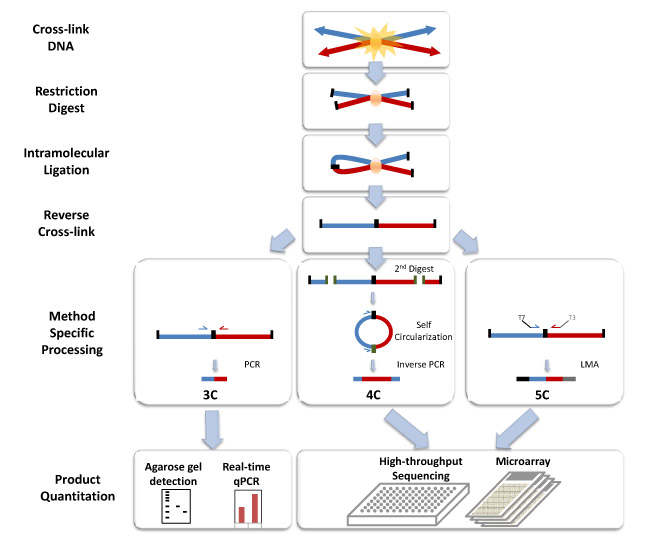
\includegraphics[scale=0.4]{./docs/Chromosome_Conformation_Capture_Technology.jpg}
    \caption{Chromosome Conformation Capture Technology}\label{3cstructure}
\end{figure}

\textbf{Hi}gh-throughput \textbf{C}hromosome conformation capture, often abbreviated to Hi-C\cite{hic}, uses high-throughput sequencing to find the nucleotide sequence of fragments and uses paired end sequencing, which retrieves a short sequence from each end of each ligated fragment. As a result, all possible pairwise interactions between fragments are tested. In other word, it can be treated as an all-vs-all method.

Although Hi-C technology is one of the most popular methods for studying 3D genome organization,the resolution of most Hi-C datasets are coarse, relatively poor at kilobase pair to megabase pair scale, which impedes more accurate analysis to get refined 3D chromatin structure. On the other hand, access to high resolution Hi-C data requires massive sequencing reads and cost, and only available in serveral tissues or cell lines. Moreover, the resolution of Hi-C data plays a major role in the effects towards downstream analysis such as TADs and chromatin loops. Therefore, computational approach is badly needed to enhancing Hi-C data resolution. 

It is a common sense that there should be a learnable mapping relationship between low resolution Hi-C data and high resolution Hi-C data, like the mapping between images and label in the field of computer vision or the relationship between words and semantic information in the field of natural language processing. Hence, we can apply neural networks on such a topic to infer high resolution Hi-C data from the low resolution Hi-C data. Previous works have proved this insight and they can be seperated into two different types, supervised or semi-supervised, according to its strategy during training.

\section{Supervised Learning Method}
In this section, I will introduce the first work, to the best of my knowledge, that applies deep learning technology to 3D genome data analysis - \textbf{HiCPlus}\cite{hicplus}.

Overall, it uses a convolutional neural network in enhancing the resolution of Hi-C data by minimizing the pixel-wise mean squared error betweem the real high resolution Hi-C data and generated Hi-C data. Such a training process is also known as supervised learning since it uses real data as label and attempts to fit the generated data to the label.

\subsection{Framework}

The Fig.\ref{hicplusframe} illustrates the framework of HiCPlus. Overall, it contains four steps:
data acquisition, down-sampling, training and predicting.

Described into pipeline, HiCPlus do as the following: Generate high resolution matrix with deeply sequenced Hi-C data. Down-sample the sequencing reads to 1/16 and resize them into the same size with former high resolution one. Train the convolutional networks to fit the model. Predict high resolution data from low resolution one.

In the following sections, I will demonstrate those steps in details.

\begin{figure}[H]
    \centering
    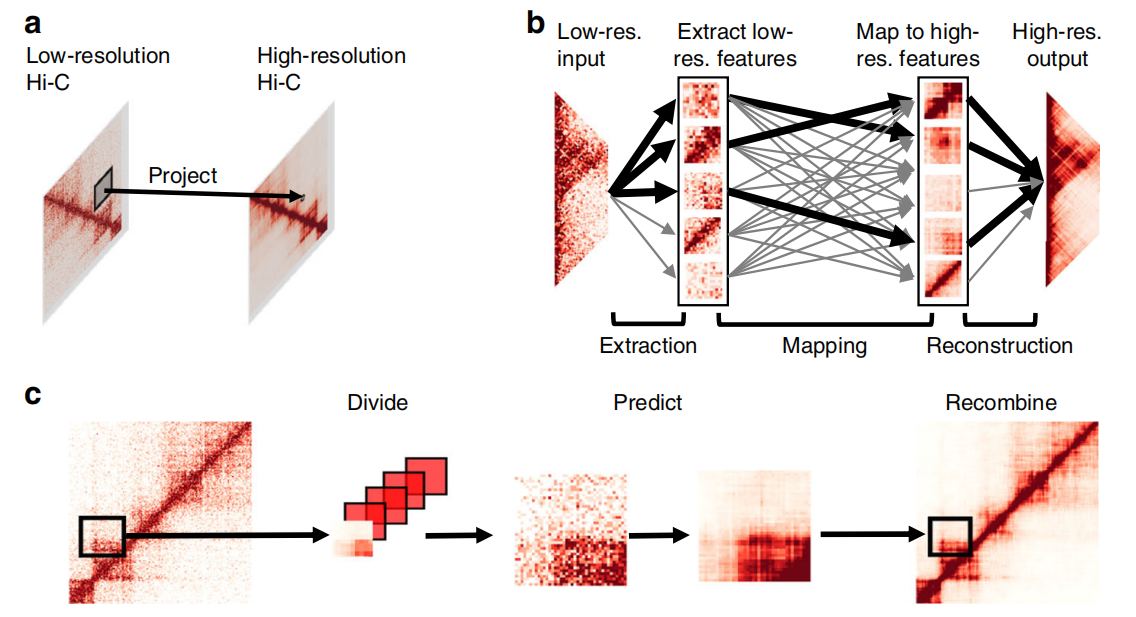
\includegraphics[scale=0.3]{./docs/hicplus_framework.jpg}
    \caption{HiCPlus Framework}\label{hicplusframe}
\end{figure}

\subsection{Data Acquisition via Down-Sampling}

As a supervised learning method, HiCPlus needs both training data and labels. As mentioned above, here we aim to learn the mapping between the low resolution HiC data to high resolution HiC data. Hence, in this problem, we should treat low resolution data as $x$ and high resolution data as $y$. Therefore, we need to get the ground truth of y and corresponding low resolution data.

To the best of my knowledge, there is no sufficient datasets for training such a mapping. That's why HiCPlus generates low resolution data from high resolution data via down-sampling, shown in Fig.\ref{downsampling}. Given the existing high resolution interaction matrix data, such as those from GM12878 or IMR90 cells, HiCPlus down-sample the sequencing reads to 1/16 - using only 1/16 or even fewer sequencing reads - and resize the result at the same resolution. Consequently, we get low resolution data with more noises and blurred patterns. Since it's generated from original high resolution data, therefore the matching relationship is well-defined so as we can train the model with generated data as input and original high resolution data as labels.

\begin{figure}[H]
    \centering
    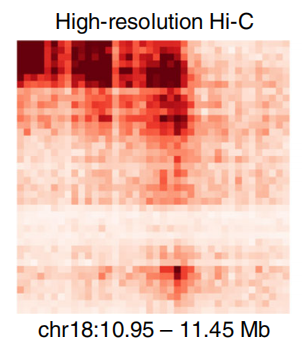
\includegraphics[scale=0.3]{./docs/hicplus_highres.png}
    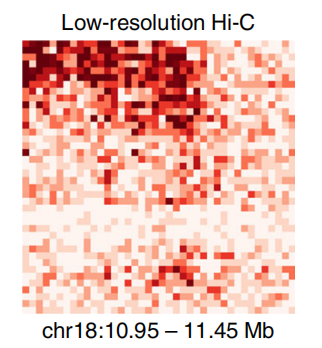
\includegraphics[scale=0.3]{./docs/hicplus_lowres.png}
    \caption{HiCPlus - Down Sampling}\label{downsampling}
\end{figure}

To note that, noises must be added when resizing the down-sampled data otherwise the mapping between low resolution data and high resolution data would be definite, which indicates that it's meaningless to use convolutional neural networks to represent such a mapping.

\subsection{Training}

Just like the usage of convolutional neural networks in classification task in the field of computer vision, HiCPlus train the model in the similar way.

\begin{figure}[H]
    \centering
    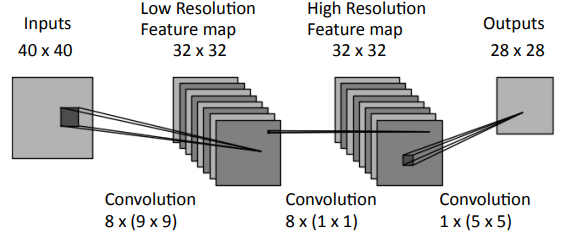
\includegraphics[scale=0.5]{./docs/hicplus_model.png}
    \caption{HiCPlus - Structure of ConvNet}\label{hicplusstruct}
\end{figure}

The structure of model is illustrated in Fig.\ref{hicplusstruct}. Using values at each position in the high resolution matrix as response  variable and its neighbouring points from the down-sampled data as the predictors, HiCPlus tries to minimize the mean squared error(MSE) at pixel-wise level. From a computer vision's perspective, a pixel in high resolution data matches a receptive fields in low resolution data. In other words, HiCPlus leverages information from surrouding regions to learn regional interaction features at each position given in the Hi-C data.


\subsection{Predicting and Enhancement}
It is an interesting practice that HiCPlus divides the entire Hi-C data into small blocks and enhances them separately. After each block of interactions are predicted, they will be merged together. 

As mentioned above, inspired by the insight from computer vision, HiCPlus becomes an end-to-end approach which makes it feasible to do the prediction on small region. Moreover, there is a strong hypothesis that the Hi-C matrix contains repeating local patterns, which makes it convincing that HiCPlus is able to predict the interaction frequency of any cell in the Hi-C matrix with the interaction frequencies from its neighbouring regions. Such a hypothesis is essential for the model of ConvNet to achieve nearly same performance on varied data. In the paper\cite{hicplus}, it is tested by the evaluation with Pearson and Spearman correlation coefficients between the predicted values and real values at each genomic distance.

The following Fig.\ref{hicplusresult} shows the efficiency of convolutional neural network model in enhancing low resolution interaction matrix.
\begin{figure}[H]
    \centering
    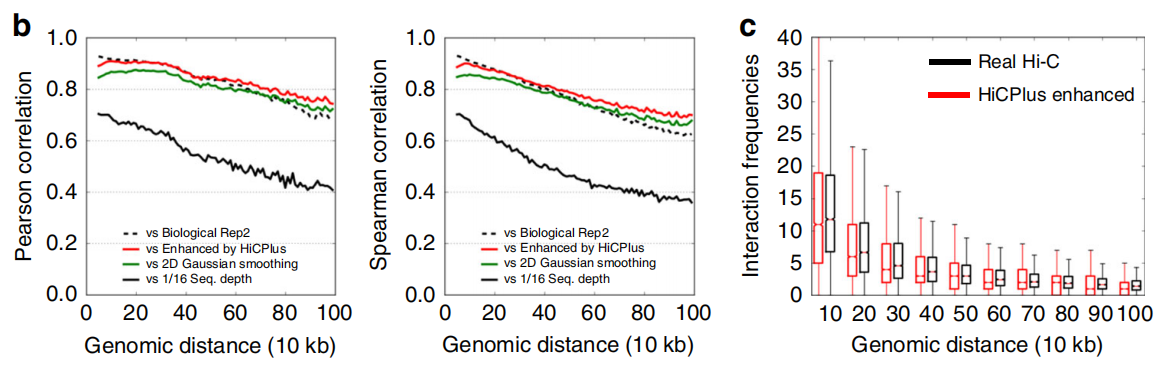
\includegraphics[scale=0.25]{./docs/hicplus_result.png}
    \caption{HiCPlus - Correlations between enhanced and real Hi-C data}\label{hicplusresult}
\end{figure}


\section{Semi-supervised Learning Method}
In this section, I will introduce second work that applies deep learning technology to 3D genome data analysis - hicGAN\cite{hicgan}.

In fact, the previous work - HiCPlus - has multiple limitations. Due to supervised training stretegy, it tends to generate Hi-C images with limited dynamic details and like most of supervised-training networks it can only be used with fixed window size. Last but not the least, HiCPlus is very sensitive to the sequencing depth of the Hi-C data.

Let's reconsider how deep learning works. In essence, it's a data-driven method which means the more data you put in the better ability of generalization you will achieve. However, as mentioned several times above, people have limited access to high resolution interaction data, which lay a dilemma here - we can do better Hi-C analysis but we can't get enough data to drive it. Therefore, the advantage of semi-supervised learning appeals charming to us.

With limited real data, semi-supervised learning teach the model how to generate realistic data, which could be the best way to augment limited Hi-C data. And the common practice of semi-supervised learning usually is generative adversarial networks\cite{gan} (also knows as GANs). Take the advantage of GANs, hicGAN present a novel framework for inferring high resolution Hi-C data from low resolution Hi-C data given the limited real data. As said in the paper, it is an effective prediction tool for enhancing resolution of Hi-C data, could shed light on the understanding of genome organization built on pair-wise interactions (all-vs-all).

\subsection{Framework}

Fig.\ref{hicganframe} illustrates the architecture of hicGAN which is a typical adversarial networks pair. Unlike HiCPlus using a single neural network, hicGAN is composed of two competitive neural networks, which are called the \textbf{Generator} and the \textbf{Discriminator}.

\begin{figure}[H]
    \centering
    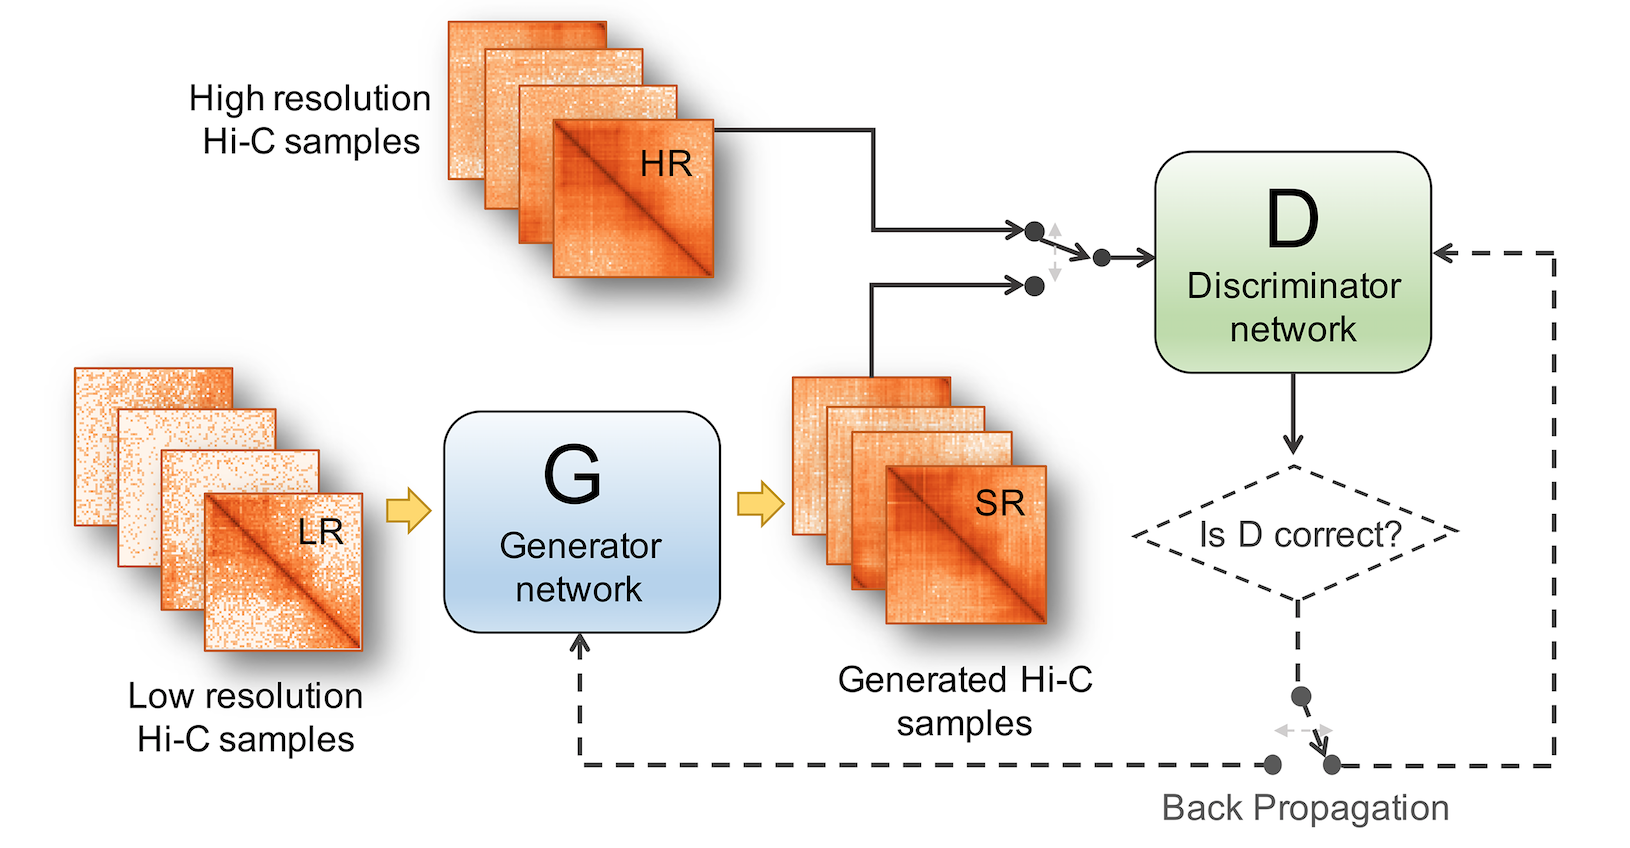
\includegraphics[scale=0.3]{./docs/hicgan_frame.png}
    \caption{hicGAN - Framework}\label{hicganframe}
\end{figure}

Since the predicting and enhancement in hicGAN are relatively similar to HiCPlus, in the following sections, I will demonstrate the generator, discriminator and training process in details seperately.

\subsection{Generator}

Take the advantage of Resnet, the generator network adopts a dual-stream residual architecture, which is proved\cite{resnet} to be effective to prevent overfitting. Moreover, same but not exactly same as HiCPlus, the generator of hicGAN is also an end-to-end network but it's a typical fully convolutional network. Thus hicGAN can handle any size of input low resolution Hi-C samples.

\begin{figure}[H]
    \centering
    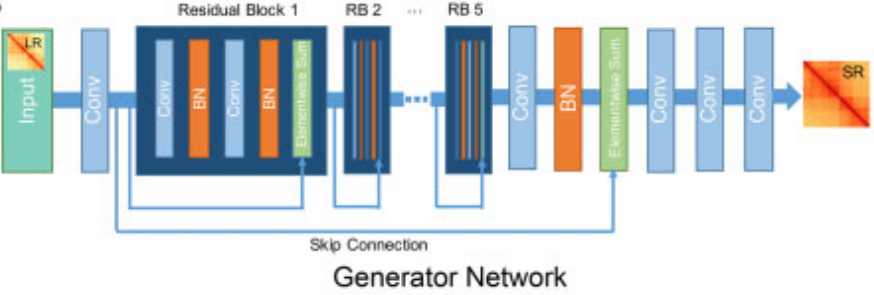
\includegraphics[scale=0.3]{./docs/hicgan_generator.png}
    \caption{hicGAN - Generator Network}
\end{figure}

\subsection{Discriminator}

The discriminator network is a classical deep convolutional neural network designed for classification task. It's trained for discerning the input high resolution data is whether real one or generated fake one.

\begin{figure}[H]
    \centering
    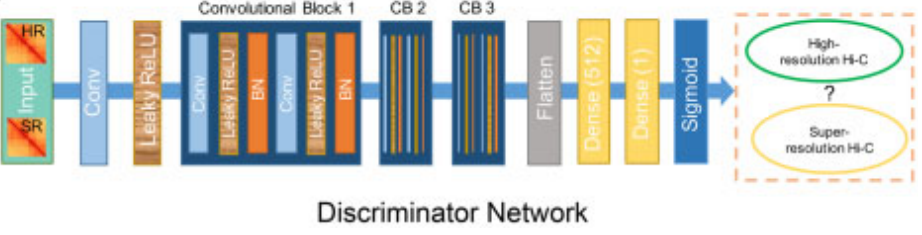
\includegraphics[scale=0.3]{./docs/hicgan_dis.png}
    \caption{hicGAN - Discriminator Network}
\end{figure}

\subsection{Adversarial Training}

The key insight of hicGAN is its adversarial training process based on game theory. Given the limited Hi-C data, we need to teach generator and discriminator to understand the essence of Hi-C data, though they achieve it in different ways. hicGAN apply adversarial training strategy for training two competitive neural network simultaneously. Generator outputs the pseudo high resolution sample given an low resolution Hi-C sample while discriminator outputs the probability (activated by sigmoid function) that the input of discriminator is a high resolution Hi-C sample. Based on game theory, the training process can be regarded as an min-max problem, which is broadly known as Nash Equilibrium.

Literally, towards this goal, generator learns to fool the discriminator while the discriminator tends to discern between the real Hi-C data and generated data. Through such a process, discriminator will potentially learns the essential feature of interactions and generator will fit itself well to real Hi-C data. Therefore, after the training converge, the generator can be used to generator amounts of interactions data. Therefore, we can solve the dilemma addressed by limited high resolution data.


\section{Discussion}
Comparing the two methods to enhance resolution of Hi-C data, I indicate that they varies in the following aspects. 

In term of motivation, HiCPlus tends to enhance Hi-C data resolution with existing features while hicGAN tries to propose computational framework to augment data regardless of its features. Theoretically, hicGAN can be applies to any type of chromatin interaction data but current public datasets are not as abundant as Hi-C datasets.

In term of training strategy, it's apparent that hicGAN is more flexible thanks to its semi-supervised strategy. Note that, it's a common sense that semi-supervised learning requires less data and gain better generalizing ability comparing to supevised learning. Given the background of limited high quality data in Hi-C analysis, semi-supervised learning has wider range of use.
Experiments also shown that correlation between generated interactions data and real data is higher in hicGAN. Thus the features of generated data are shared across different cell types which shuld be highly related to the crucial functions of 3D genome organization.

However, deep learning methods in Hi-C analysis is not an panacea. Due to the unexplictable property of neurons in neural network, it's still somehow difficult to interpret exact features the model has learnt. If so, it would be easy to decipher complex mechanism within 3D genome organization.

\section*{Acknowledgments}
I would like to express my sincere thanks to Prof. Shao Li as well as Dr. Siyu Hou, who helped us to gain a comprehensive overview of computational biology in the past semester.

\begin{thebibliography}{99}
    \bibitem{hicplus}Zhang,Y. et al. (2018) Enhancing Hi-C data resolution with deep convolutional neural network HiCPlus. Nat. Commun., 9, 750.

    \bibitem{resnet}Kaiming He and Xiangyu Zhang and Shaoqing Ren and Jian Sun. (2015). Deep Residual Learning for Image Recognition.

    \bibitem{gan}Goodfellow,I. et al. (2014) Generative adversarial nets. In: Advances in Neural Information Processing Systems, Curran Associates, Inc. Montreal, Quebec, Canada, Dec 8, 2014 – Dec 13, 2014, pp. 2672–2680.

    \bibitem{hic}Lieberman-Aiden,E. et al. (2009) Comprehensive mapping of long-range interactions reveals folding principles of the human genome. Science, 326,289–293

    \bibitem{hicgan}Liu, Q.; Lv, H.; Jiang, R. hicGAN infers super resolution Hi-C data with generative adversarial networks. Bioinformatics 2019, 35, i99–i107.

    \bibitem{3c}https://en.wikipedia.org/wiki/Chromosome\_conformation\_capture
\end{thebibliography}



\end{document}